\chapter{醫學詞彙專題 - Medical Glossary}
\section{醫學詞彙構詞法 (未完待續)}
\subsection{人體主要器官前後綴}
\begin{itemize}
  \itemsep0em
  \item 心: heart \hilight{cardia$\sim$} cardial cardium / carditis / cardiology
  \item 腦: brain \hilight{encepholo$\sim$} cerebral cerebrum / encephalitis / encephalology
  \item 肺: lung \hilight{pulmo$\sim$} pulmonary pulmontiis / pulmonectomy / pulmonology
  \item 肝: liver \hilight{hepato$\sim$} hepatic hepatitis / hepatobiliary / hepatology
  \item 胃: stomach \hilight{gastro$\sim$} gastric gastritis / gastrointestinal / gastrology
  \item 膽: gallbladder \hilight{chole$\sim$} biliary holecystitis / cholinergic / cholecystectomy
  \item 腸: intestine \hilight{entero$\sim$} intestinal enteritis / enterectomy / enterology
  \item 脾: spleen \hilight{splen$\sim$} splenic splenitis / splenectomy / splenology
  \item 胰: pancreas \hilight{pancreato$\sim$} pancreatic pancreatitis / pancreatectomy
  \item 腎: kidney \hilight{nephro$\sim$} renal / nephric nephritis / nephropathy / nephrology
\end{itemize}

\subsection{人體系統 / 器官前後綴}
\begin{itemize}
  \itemsep0em
  \item 血: blood \hilight{hemo$\sim$} / hemato hematology / hemoglobin / hematoma
  \item 血管: vessel \hilight{vaso$\sim$} vasopressor / cardiovasology / verebrovascular
  \item 靜脈: vein \hilight{veno$\sim$} venography / intravenous / venoconstriction
  \item 動脈: artery \hilight{arterio$\sim$} arteriology / arteriole / arteriosclerosis
  \item 肌: muscle \hilight{myo$\sim$} mycology / myositis / myocarditis
  \item 髓: marrow \hilight{myel$\sim$} / \hilight{myelo$\sim$} myelocyte / myelitis / myeloma
  \item 神經: nerve \hilight{neur$\sim$} / \hilight{neyro$\sim$}  neurology / neuritis / neuron
  \item 細胞 cell \hilight{cyto$\sim$} / \hilight{$\sim$cyte} cytology / cytoma / leukocyte
  \item 尿 urine \hilight{uro$\sim$} / \hilight{ur$\sim$} urology / urosurgery / urogenital
  \item 體 body \hilight{somato$\sim$} / some somatology / somatopsychic / chromosome
\end{itemize}

\subsection{與疾病和疾患有關的前後綴}
\begin{itemize}
  \itemsep0em
  \item 相反 \hilight{dis$\sim$} disease / disorder / disability 
  \item 困難/障礙 \hilight{dys$\sim$} dysfunction / dyspepsia / dyspnea 
  \item 不良 \hilight{mal$\sim$} malfunction / malnutrition / malpractice 
  \item 炎症 \hilight{$\sim$itis} appendicitis / bronchitis / arthritis 
  \item 瘤/塊 \hilight{$\sim$oma} lymphoma / adenoma / hematoma 
  \item 血症 \hilight{$\sim$emia} leukemia / septisemia / bacteremia 
  \item 痛 \hilight{$\sim$algia} / \hilight{$\sim$algesia} / \hilight{alge$\sim$} / \hilight{algo$\sim$} analgesia / hypoalgesia / algometer 
  \item 麻痹 \hilight{$\sim$plegia} hemipleia / pamplegia / myoplegia 
  \item 流出 \hilight{$\sim$rrhea} diarrhea / hypermenorrhea / rhinorrhea 
  \item 壞死 \hilight{$\sim$necrosis} \hilight{necro$\sim$} / \hilight{necr$\sim$} hepatonecrosis / myonecrosis / necrospermia 
  \item 結石 \hilight{litho$\sim$} / \hilight{$\sim$lith} lithiasis / lithogenesis / cholelithes
\end{itemize}

\subsection{與顏色有關的前綴}
\begin{itemize}
  \itemsep0em
  \item 色 color \hilight{chrom$\sim$} / \hilight{chromo$\sim$} chromosome / chromatin / chromatometer
  \item 紅 red \hilight{erythro$\sim$} erythrocyte / erythrocyturia / erythrometer
  \item 白 white \hilight{leuko$\sim$} leukocyte / leukemia / leukocytuira
  \item 黑 black \hilight{melano$\sim$} melena / melanoma / melanoderma
  \item 黃 yellow \hilight{xantho$\sim$} xanthopsin / xanthosis/xanthoma
  \item 藍 blue \hilight{cyan$\sim$} / cyano cyanosis / cyanopsia / cyanemia
  \item 紫 violet / purple
  \item 綠 green
  \item 棕 brown brown mixture / brown ring
  \item 橙 orange Victoria orange / ethyl orange / orange G
  \item 粉紅 pink oink frothy sputum
  \item 緋紅 crimson
  \item 青銅 bronzed bronzed diabetes
\end{itemize}

\subsection{與數字有關的前綴}
\begin{itemize}
  \itemsep0em
  \item 一:(單) \hilight{mono$\sim$} / \hilight{uni$\sim$} monomer / monoclone / carbon monoxide / unidirectional 
  \item 二: \hilight{bi$\sim$} / \hilight{di$\sim$} bilateral / biphasiccarbon dioxide / dipeptide 
  \item 三: \hilight{tri$\sim$} trilateral / triphasic / trigeminal nerve 
  \item 四: \hilight{tetra$\sim$} tetramer / tetracycline / tetraplegia 
  \item 五: \hilight{penta$\sim$} pentagon / pentachromic / pentachloride 
  \item 六: \hilight{hexa$\sim$} hexachromic / benzene hexachloride / hexacycliccompiund 
  \item 七: \hilight{hepta$\sim$} heptachromic / heptaploid / heptavalent 
  \item 八: \hilight{octa$\sim$} octahedral / octal system 
  \item 九: \hilight{nona$\sim$} nonapeptide / nonagon 
  \item 十: \hilight{deca$\sim$} decade / decagram / decaliter
\end{itemize}

\section{實習醫生格蕾出現的單詞(不含DI課上已學過的)}
\begin{multicols}{2}
\begin{itemize}
  \itemsep0em
  \item ICU: Intensive Care Unit (重症病房)
  \item DNR: Do Not Resuscitate (病情惡化不進行搶救和用機器維持生命)
  \item Surgeon / Surgery: 外科醫生 / 外科手術
  \item O.R.: Operating Room (手術室)
  \item CPR: Cardiopulmonary Resuscitation (心肺復蘇)
  \item page: (通過擴音器、傳呼機等)呼叫
  \item Scrubs: 刷手服. 也就是他們穿的那身藍衣服, 外科醫生刷手時穿的, 手術時外面再罩一件手術衣
  \item Chief Resident: 住院總醫師
  \item On Call Room: 值班室
  \item Glasgow Coma Scale 格拉斯哥昏迷指數\footnote{詳情請見:\url{https://en.wikipedia.org/wiki/Glasgow_Coma_Scale}} (GCS)
  \item Central Line 中央靜脈置管
  \item Neurocysticercosis: 腦囊蟲病 (Worm in the brain)
  \item Pituitary Gland: 腦垂體
  \item Frontal Lobe: 額葉
  \item Temporal Lobe 顳葉
  \item Third Ventricle: 第三腦室
  \item Salpingectomy: 輸卵管切除術
  \item Ovary: 卵巢
  \item LP (Lumber Puncture): 腰椎穿刺
  \item Bone Marrow Transplantation: 骨髓移植
  \item Leukemia: 白血病
  \item Adenosine: 腺苷 (室上速常用藥,不過現在已經很少用了)
  \item Coronary Artery: 冠狀動脈
  \item Morgue: 停屍房 / 太平間
  \item Nasal Lavage: 鼻腔灌洗
  \item Blood Culture: 血培養
  \item Hematology: 血液學
  \item Aorta: 主動脈
  \item Amioderon: 胺碘酮 (各型心律失常常用藥)
  \item PS endoscopy: 並不是單指胃鏡,是泛指所有的``腔鏡"
  \item LVAD Left Ventricular Assistant Device: 左心室起搏輔助裝置 (起搏器)
  \item Dual Chamber Pacemaker: 雙腔起搏器
  \item scalpel: 手術刀
  \item gurney: 推床
  \item scrub in: 參與手術的另類講法
  \item suction: 手術室抽吸創口周圍的血,使得視野更清晰
  \item pit: 急診室
  \item Chopper: 直升機
  \item Dressing: 換包扎
  \item E.R (Emergency Room): 急診室
  \item scalpel: 手術刀
  \item clincal trial- meredith和derek往腦瘤里注射病毒是一種臨床試驗
  \item Neuropharmacology: 藥理學
  \item valve: 瓣膜
  \item cardiac catheterisation: 心臟導管插入
  \item pericardiocentesis: 心包穿刺
  \item congenital heart disease: 先天性心臟病
  \item I.V.S: 靜脈滴注
  \item catheter: 導尿管
  \item contraction: 宮縮
  \item v-fib: 室顫
  \item pica: 異食症
  \item third-degree burn: 三級燒傷
  \item pathology: 病理學
  \item dialysis: 透析
  \item nerve graft: 神經移植
  \item hemiglossectomy: 半舌切割術
  \item atropine: 阿托品
  \item cardiac arrest: 心臟停止跳動
  \item hydrocephalus: 腦水腫
  \item spinal fluid: 脊髓液
  \item bacterial endocarditis: 細菌性心內膜炎
  \item cortisone: 腎上腺皮質激素
  \item asystole: 心搏停止
  \item brain dead: 腦死亡
  \item hematoma: 血腫
  \item angioplasty: 血管成形術
  \item vital signs stable: 生命跡象穩定
  \item forceps: 鉗子
\end{itemize}
\begin{itemize}
    \itemsep0em
    \item 實習醫生: intern
    \item 住院醫生: resident doctor 
    \item 主治醫生: doctor in charge / attending doctor 
    \item 草藥醫生: herb doctor
    \item 產科醫生: obstetrician
    \item 開業醫生: practicing doctor
    \item 外科醫生 / 內科醫生: surgeon / physician
    \item 皮膚科醫生 / 整形外科醫生: dermatologist / plastic surgeon
    \item 腫瘤科醫生: oncologist
\end{itemize}
\begin{itemize}
    \itemsep0em
    \item Be flexible: 通融點
    \item That is the gravy: 那時額外的獎勵
    \item Lighten up: 放輕鬆
    \item It is very homework:非常典型
  \item Discharge paper: 出院文件
    \item You are an ass: 你是個混蛋
    \item I will get you covered: 我會罩著你
    \item My lips are sealed: 我守口如瓶
    \item Do not make a deal about it: 不要小題大做
\end{itemize}
\end{multicols}

\section{身體部位和器官}
\subsection{人的器官一覽}
\begin{center}
  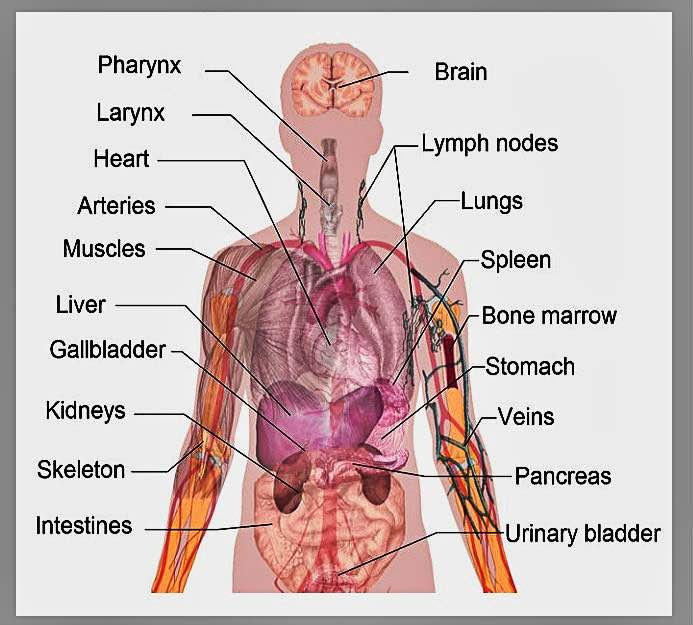
\includegraphics[scale=0.4]{pics/in-body}
\end{center}

\subsection{和頭面部有關的詞}
\begin{multicols}{3}
\begin{itemize}
  \itemsep0em
  \item beard: 鬍鬚
  \item moustache: 鬍子
  \item cheek: 臉頰
  \item chin: 下巴
  \item eyebrow / eyelash: 眉毛 / 睫毛
  \item eardrum / earlobe: 耳膜 / 耳垂
  \item eyelid: 眼瞼
  \item forehead: 額頭
  \item freckles: 雀斑
  \item jaw: 下頜
  \item lip: 嘴唇
  \item nostril: 鼻孔
  \item tongue: 舌頭
  \item wrinkles: 皺紋
\end{itemize}
\end{multicols}

\subsection{和上半身有關的詞}
\begin{multicols}{3}
\begin{itemize}
  \itemsep0em
  \item Adam's apple: 喉結
  \item armpit: 腋窩
  \item breast / chest: 胸 / 胸口
  \item elbow: 肘
  \item fingernail: 指甲
  \item forearm: 前臂
  \item knuckle: 指關節
  \item navel / belly button: 肚臍
  \item neck: 脖子
  \item nipple: 乳頭
  \item lower back: 腰
  \item wrist: 手腕關節
\end{itemize}
\end{multicols}

\subsection{和下半身有關的詞}
\begin{multicols}{3}
\begin{itemize}
  \itemsep0em
  \item ankle: 腳踝
  \item anus: 肛門
  \item belly: 肚子
  \item bottom (俚語: bum): 屁股
  \item buttocks: 臀部
  \item calf: 小腿
  \item genitals: 生殖器
  \item groin: 腹股溝
  \item heel: 腳後跟
  \item hip: 臀部
  \item leg: 腳
  \item pubic hair: 陰毛
  \item shin: 脛骨
  \item sole: 腳掌
  \item testicles: 睪丸
  \item thigh: 大腿
  \item toe: 腳趾
  \item toenail: 腳趾甲
  \item vagina: 陰道
\end{itemize}
\end{multicols}

\subsection{和眼部有關的詞}
\begin{multicols}{3}
\begin{itemize}
  \itemsep0em
  \item cornea: 角膜
  \item eye socket: 眼窩
  \item eyeball: 眼球
  \item iris: 虹膜
  \item retina: 視網膜
  \item pupil: 瞳孔
\end{itemize}
\end{multicols}

\subsection{和體內有關的詞}
\begin{multicols}{3}
\begin{itemize}
  \itemsep0em
  \item Achilles tendon: 跟腱
  \item artery: 動脈
  \item appendix: 闌尾
  \item bladder: 膀胱
  \item blood vessel: 血管
  \item cartilage: 軟骨
  \item colon: 結腸
  \item gall bladder: 膽囊
  \item intestines: 腸道
  \item large intestine: 大腸
  \item small intestine: 小腸
  \item kidneys: 腎臟
  \item ligament: 韌帶
  \item liver: 肝
  \item lungs: 肺
  \item oesophagus: 食道
  \item pancreas: 胰腺
  \item organ: 器官
  \item prostate gland: 前列腺
  \item rectum: 直腸
  \item spleen: 脾
  \item stomach: 胃
  \item tendon: 腱
  \item tonsils: 扁桃體
  \item vein: 血管
  \item windpipe: 氣管
  \item womb / uterus: 子宮
\end{itemize}
\end{multicols}

\subsection{和骨骼有關的詞}
\begin{multicols}{3}
\begin{itemize}
  \itemsep0em
  \item collarbone / clavicle: 鎖骨
  \item thigh bone / femur: 股骨
  \item humerus: 肱骨
  \item kneecap: 膝蓋骨
  \item pelvis: 骨盆
  \item rib: 肋骨
  \item rib cage: 胸腔
  \item skeleton: 骨架
  \item skull: 頭蓋骨
  \item spine / backbone: 脊柱
  \item vertebra (複數vertebrae): 椎骨
\end{itemize}
\end{multicols}

\subsection{和體液有關的詞}
\begin{multicols}{3}
\begin{itemize}
  \itemsep0em
  \item bile: 膽汁
  \item blood: 血
  \item mucus: 黏液
  \item phlegm: 痰
  \item saliva / spit: 唾液
  \item semen: 精液
  \item sweat / perspiration: 汗
  \item tears: 眼淚
  \item urine: 尿液
  \item vomit: 嘔吐物
\end{itemize}
\end{multicols}

\subsection{和官能有關的詞}
\begin{multicols}{3}
\begin{itemize}
  \itemsep0em
  \item smell: 嗅覺
  \item touch: 觸覺
  \item sight: 視覺
  \item hearing: 聽覺
  \item taste: 味覺
  \item to smell: 聞
  \item to touch: 觸
  \item to see: 看
  \item to hear: 聽
  \item to taste: 嘗
\end{itemize}
\end{multicols}

\section{人體的各種"系統" (以下所有詞後面加System)}
\begin{multicols}{3}
\begin{itemize}
  \itemsep0em
  \item Digestive $\sim$: 消化系統 
  \item Excretory $\sim$: 排泄系統
  \item Integumentary $\sim$: 皮膚系統
  \item Cardiovascular $\sim$: 心血管系統
  \item Circulatory $\sim$: 循環系統
  \item Endocrine $\sim$: 內分泌系統
  \item Immune $\sim$: 免疫系統
  \item Lymphatic $\sim$: 淋巴系統
  \item Muscular $\sim$: 肌肉組織系統
  \item Musculoskeletal $\sim$: 肌肉骨骼系統
  \item Nervous $\sim$: 神經系統
  \item Reproductive $\sim$: 生殖系統
  \item Respiratory $\sim$: 呼吸系統
  \item Skeletal $\sim$: 骨骼系統
  \item Urinary $\sim$: 泌尿系統
\end{itemize}
\end{multicols}

\section{常用醫學名詞}
\begin{multicols}{3}
\begin{itemize}
  \itemsep0em
  \item 健康診斷: General Check-up / Physical Examination
  \item 入院: Admission to Hospotial
  \item 退院: Discharge from Hospital
  \item 病例: Clinical History
  \item 預防: Prevention
  \item 呼吸: Respiration
  \item 便通: Bowel Movement
  \item 便: Stool
  \item 脈搏: Pulse, Pulsation
  \item 脈搏數: Pulse Rate
  \item 切除: Resectionlie
  \item 洗淨: Irrigation
  \item 紅外線: Ultra Red-Ray
  \item 慢性的: Chronic
  \item 急性的: Acute
  \item 體格: Build
  \item 遺傳: Heredity
  \item 免疫: Immunity
  \item 血清: Serum
  \item 流行性的: Epidemic
  \item 潛伏期: Incubation Period
  \item 濾過性病毒: Virus
  \item 消毒: Sterilization
  \item 洗腸: Enema
  \item 結核反映: Tuberculin Reaction
  \item 華氏: Fahrenheit
  \item 攝氏: Celsius, Centigrade
\end{itemize}
\end{multicols}

\section{和疾病有關的詞}
\begin{itemize}
  \itemsep0em
  \item 膽結石: gall stone
  \item 結核: TB $\xrightarrow{\text{全稱, 不要翻譯成肺結核}}$ tuberculosis
  \item 肺結核: Pulmonary TB, 肺炎: pulmonitis (tis結尾大多是炎症) / pneumonia
  \item 傳染病: contagious / infectious disease
  \item 胸片: chest X-ray
  \item 細菌: germ / bacteria
  \item 肺: lungs, (大/小)腸道: (\hilight{large}/small) intestine / bowel
  \item 胃潰瘍: gastric ulcer
  \item 潛伏期: latent period / incubation
  \item (慢性的)支氣管炎: (chronic) bronchitis
  \item 膽固醇: cholesterol
  \item ``三高":
  \begin{enumerate}
    \itemsep0em
    \item Hypertension: 高血壓
    \item Hyperglycaemia: 高血糖 (帶ae的一般和血有關, 以ia結尾的一般指病)
    \item Hyperlipidaemia: 高血脂 (lipid一般指脂肪, 比fat指的要小)
  \end{enumerate}
\end{itemize}

\section{不同的疼法}
\begin{multicols}{3}
\begin{itemize}
  \itemsep0em
  \item 頭疼: headache
  \item 激痛: severe pain
  \item 急性疼痛: acute pain
  \item 燒痛 / 灼燒感: burning pain / sensation
  \item 刺痛: stabbing pain
  \item 抽痛 / 一跳一跳地痛: throbbing pain
  \item 一陣一陣痛: intermittent pain
  \item 產痛: labour pain
  \item 劇痛: sharp pain
  \item 頑痛: persistent pain
  \item 隱隱作痛: dull pain
  \item 撕裂痛: splitting / tearing pain
  \item 痙攣痛: crampy pain
  \item 脹痛: bloating pain
  \item 輕痛: slight Pain
  \item 戳痛: piercing pain
  \item 壓痛: tenderness
  \item 持續痛: continuous pain
  \item 針扎似的痛: prickling pain
  \item 不能忍受的痛: excruciating pain
  \item 腫痛: swelling pain
  \item (腹部)絞痛: colic
  \item 刺麻感(不屬於痛): pin / needles
\end{itemize}
\end{multicols}

\section{不同的麻醉方式}
\begin{multicols}{2}
\begin{itemize}
  \itemsep0em
  \item 麻醉師: anaesthetist
  \item 全麻: general anaesthetic
  \item 局麻: local anaesthetic
  \item 脊麻: spinal anaesthetic
  \item 硬膜外麻: epidural anaesthetic\footnote{硬膜外間隙阻滯麻醉,即將局麻藥注入硬膜外腔,阻滯脊神經根,暫時使其支配區域產生麻痹,稱為硬膜外間隙阻滯麻\\醉,簡稱為硬膜外阻滯。}
\end{itemize}
\end{multicols}

\section{不同的治療方式}
\mybox{\centering \textbf{注意}: 以下單詞去掉therapy結尾即表簡稱}
\begin{multicols}{2}
\begin{itemize}
  \itemsep0em
  \item physiotherapy: 物理治療
  \item chemotherapy: 化學治療
  \item radiotherapy: 放射治療
  \item electrotherapy: 電療
  \item hydrotherapy: 水療\footnote{皮膚燒傷, 行動不便的時候採取的治療}
  \item $\sim$therapist: $\sim$治療師
\end{itemize}
\end{multicols}

\section{不同的醫院}
\begin{multicols}{2}
\begin{itemize}
  \itemsep0em
  \item children's hospital: 兒童醫院
  \item general hospital, polyclinic: 綜合醫院
  \item leprosarium: 麻風病院
  \item maternity hospital / lying-inhospital: 產科醫院
  \item mental hospital, mental home: 精神病院
  \item obstetrics and gynecology hospital: 婦產醫院
  \item plastic surgery hospital: 整形外科醫院
  \item stomatological hospital: 口腔醫院
  \item tuberculosis hospital: 結核病醫院
  \item tumour hospital: 腫瘤醫院
  \item clinic: 診療所
  \item first-aid station: 急救站
  \item polyclinic: 聯合診療所
  \item quarantine station: 防疫站(檢疫所)
  \item rest home: 休養所
  \item sanatorium: 療養院
\end{itemize}
\end{multicols}

\section{不同的醫院科室}
\begin{multicols}{2}
\begin{itemize}
  \itemsep0em
  \item medical department: 內科
  \item surgical department: 外科
  \item anaesthesiology department: 麻醉科
  \item cardiology department: 心臟病科
  \item dental department: 牙科
  \item dermatology department, skin department: 皮膚科
  \item department of cardiac surgery: 心臟外科
  \item department of cerebral surgery: 胸外科
  \item general surgery: 普通外科
  \item neurology department: 神經科
  \item neurosurgery department: 精神外科
  \item obstetrics \& gynecology department: 婦產科
  \item ophthalmology department: 眼科
  \item orthopedic surgery department: 矯形外科
  \item orthopedics department: 骨科
  \item otorhinolaryngological department: 耳鼻喉科
  \item paediatrics department: 小兒科
  \item pathology department: 病理科
  \item plastic surgery: 整形外科
  \item psychiatry department: 精神病科
  \item thoracic surgery department: 腦外科
  \item traumatology department: 創傷外科
  \item urology department: 泌尿科
  \item X-ray department: 放射科
  \item registration office: 掛號處
  \item out-patient department, OPD: 門診部
  \item in-patient department: 住院部
  \item nursing department: 護理部
  \item consulting room: 診室
  \item waiting room: 候診室
  \item admitting office: 住院處
  \item emergency room: 急診室
  \item operation / theatre: 手術室
  \item laboratory: 化驗室
  \item blood bank: 血庫
  \item pharmacy, dispensary: 藥房
  \item ward: 病房
  \item medical ward: 內科病房
  \item surgical ward: 外科病房
  \item maternity ward: 產科病房
  \item isolation ward: 隔離病房
  \item observation ward: 觀察室
  \item hospital bed: 病床
\end{itemize}
\end{multicols}

\section{和暈車暈船有關的症狀}
\begin{itemize}
  \itemsep0em
  \item 臉發白: pale face
  \item 胸悶: chest \hilight{tightness}
  \item 嗜睡: drowsiness
  \item 疲憊: \hilight{fatigue}
\end{itemize}

\section{和皮膚病有關的詞}
\begin{multicols}{3}
\begin{itemize}
  \itemsep0em
  \item 痔, 胎記: \hilight{mole}
  \item 色素沈積 pigmentation
  \item 黑素瘤: melanoma (noma結尾指瘤)
  \item 粉刺: pimple
  \item 痂: scab
  \item 斑: dark spot
  \item 黑眼圈: dark circle
  \item 痘: acne
  \item 水泡: blister
  \item 疣: wart
  \item 酒糟鼻: brandy nose
\end{itemize}
\end{multicols}

\section{和醫療有關的詞}
\begin{itemize}
  \itemsep0em
  \item 公費醫療: bulk billing
  \item 轉診信: referral letter (不要翻譯成推薦信)
  \item 註冊醫生: registrar $\xrightarrow{\text{轉正+變得牛逼}}$ 主任醫生: consultant
  \item 中醫/西醫: \hilight{traditional} Chinese medicine / conventional medicine
  \item 心/腦電圖: ECG / EEG
  \item 骨密度測試: bone density test
\end{itemize}